\documentclass[12pt]{article}
\usepackage[a4paper,landscape,margin=2cm]{geometry}

\usepackage{import}

\import{./}{preamble.tex}
\import{./}{songcolumns-3.tex}

\begin{document}

\import{./}{titlepage.tex}

\begin{center}
  \begin{minipage}[t][0.2\textheight][t]{0.8\textwidth}
    \centering
    \textbf{\sffamily \LARGE Beyond Fur, 2020\hfill}%
    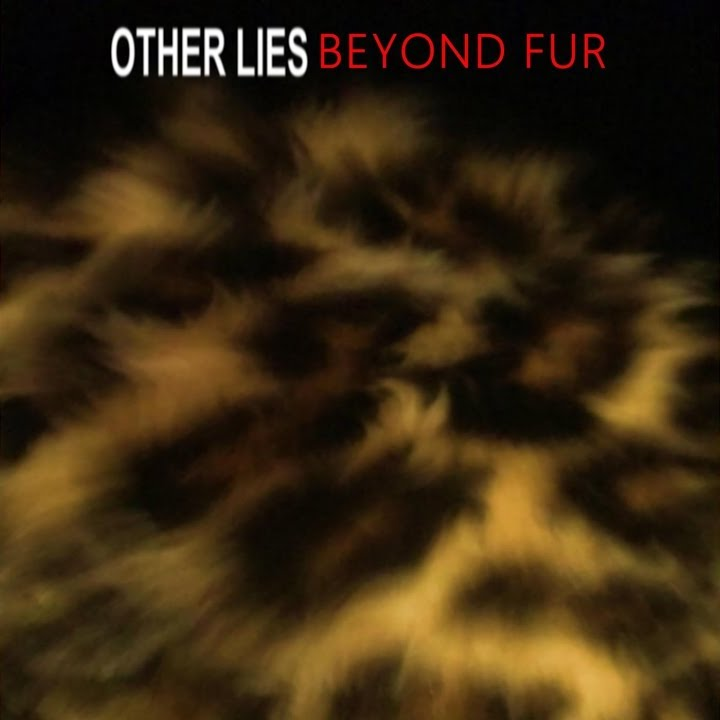
\includegraphics[height=0.2\textheight,valign=t]{1-Beyond-Fur/beyond-fur.jpg}
  \end{minipage}

  \vspace{1em}
  
  \begin{minipage}[t][0.5\textheight][t]{\textwidth}
    \centering
    \resizebox{0.8\textwidth}{!}{% use resizebox with line width
      \rowcolors{2}{gray!10}{white}
      \begin{tabular}{>{\sffamily}r>{\bfseries \sffamily}l>{\sffamily}l>{\sffamily}r}
        %%\rowcolor{gray!15}
        \# & Title                       & Key         & Tempo \\
        \hline
        1  & The The Incense of Valletta & C           & 92    \\
        2  & Hallucinogenic              & E           & 92    \\
        3  & My Favourite Scarlet        & F\sharp$_m$ & 140   \\
        4  & The Obsession With Control  & E$_m$       & 130   \\
        5  & Gin Lane                    & E$_m$       & 80    \\
        6  & Vague Idols                 & C           & 113   \\
        7  & Sandman Sabotage            & C           & 113   \\
        8  & Real Red Nail Polish        & C           & 113   \\
        9  & Tattooed Indian Robber      & C           & 113   \\
        10 & Of Human Bondage            & A           & 120   \\
      \end{tabular}%
    }
  \end{minipage}
\end{center}

\pagebreak
\import{./1-Beyond-Fur/}{songs.tex}

\pagebreak

\begin{center}
  \begin{minipage}[t][0.2\textheight][t]{0.8\textwidth}
    \centering
    \textbf{\sffamily \LARGE Surfacing, 2022\hfill}%
    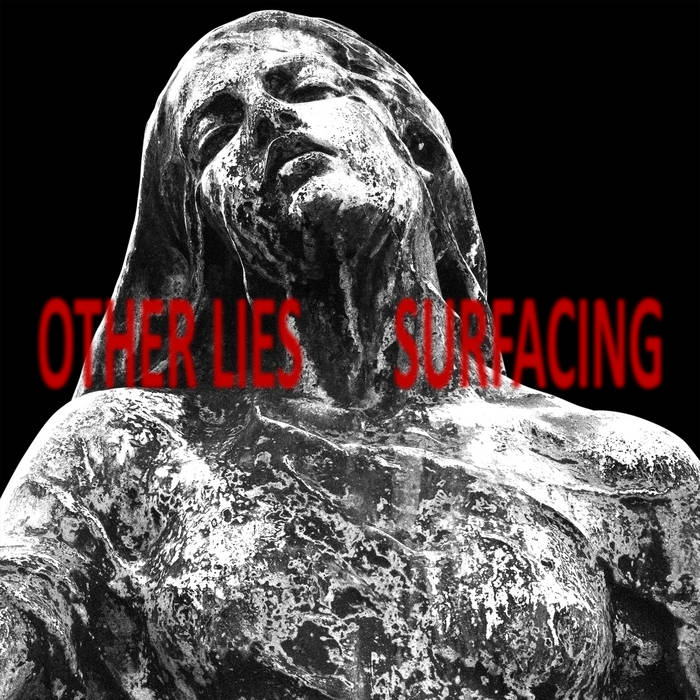
\includegraphics[height=0.2\textheight,valign=t]{2-Surfacing/surfacing.jpg}
  \end{minipage}

  \vspace{1em}
  
  \begin{minipage}[t][0.5\textheight][t]{\textwidth}
    \centering
    \resizebox{0.8\textwidth}{!}{% use resizebox with line width
    \rowcolors{2}{gray!10}{white}
    \begin{tabular}{>{\sffamily}r>{\bfseries \sffamily}l>{\sffamily}l>{\sffamily}r}
      %%\rowcolor{gray!15}
      \# & Title               & Key         & Tempo \\
      \hline
      1  & Belle of the Ball   & C           & 113   \\
      2  & The Bath            & B\flat      & 128   \\
      3  & Dead End For Delhia & C           &       \\
      4  & Stars on Black      & A$_m$       & 100   \\
      5  & Vibrator            & D$_m$       & 113   \\
      6  & Kawasaki            & F\sharp$_m$ & 90    \\
      7  & Ayurveda            &             & 127   \\
      8  & Ruin Porn           &             &       \\
      9  & In Candesenza       & E$_m$       & 130   \\
      10 & Sequoia             & D           & 130   \\
    \end{tabular}%
    }
  \end{minipage}
\end{center}

\pagebreak
\import{./2-Surfacing/}{songs.tex}

\pagebreak

\begin{center}
  \begin{minipage}[t][0.2\textheight][t]{0.8\textwidth}
    \centering
    \textbf{\sffamily \LARGE Ultrablanc, 2025\hfill}%
    \includegraphics[height=0.2\textheight,valign=t]{3-Ultrablanc/ultrablanc.png}
  \end{minipage}

  \vspace{1em}
  
  \begin{minipage}[t][0.5\textheight][t]{\textwidth}
    \centering
    \resizebox{0.8\textwidth}{!}{% use resizebox with line width
    \rowcolors{2}{gray!10}{white}
    \begin{tabular}{>{\sffamily}r>{\bfseries \sffamily}l>{\sffamily}l>{\sffamily}r}
      %%\rowcolor{gray!15}
      \# & Title                & Key    & Tempo \\
      \hline
      1  & The Color Of Thunder    & A     & 115 \\
      2  & The Whirlwind of Lovers & G$_m$ & 108 \\
      3  & Bones                   & D     & 90  \\
      4  & Paramount               & D     & 105 \\
      5  & Holy Burn               & A$_m$ & 80  \\
      6  & Voiles                  & B$_m$ & 95  \\
      7  & Mottainai               & B$_m$ & 105 \\
      8  & Vanity Rewinds          & E$_m$ & 80  \\
      9  & Teens 4 Today           & E     & 127 \\
      10 & The Last Embrace        & E$_m$ & 80  \\      
    \end{tabular}%
    }
  \end{minipage}
\end{center}
\pagebreak
\import{./3-Ultrablanc/}{songs.tex}

\end{document}
